\documentclass[11pt,a4paper]{article}
\usepackage[margin=25mm]{geometry}
\usepackage{fontspec,unicode-math,amsmath,booktabs,graphicx,hyperref}
\setmainfont{STIXGeneral}\setmathfont{STIX Two Math}
\setlength{\parindent}{0pt}\setlength{\parskip}{6pt}
\title{Supported kernels and affine constructions}
\author{Nine-original manuscript comparison}\date{}
\begin{document}\maketitle
The nine complete originals contain 273,937 characters. The entire common paper and all nine complete applications contain 202,265 characters. The primary whole-topic comparison is
\[
 R=\frac{\sum_{i=1}^{9}c(S_i)}{c(U)+\sum_{i=1}^{9}c(A_i)}
 =\frac{273937}{66140+136125}
 =1.354347.
\]
Here $c$ counts characters excluding whitespace after NFC normalization of the accepted selected and calibrated PDF extraction. This convention was fixed before evaluation and preserves the prior A coordinate. It measures the length of these manuscripts, not the least possible proof length or historical originality.

All 131 source pages, the whole 23-page common paper and all 56 application pages are charged. Titles, abstracts, full proofs, tables, references, author addresses and extractable figure labels remain. There is no common-theory import free of charge, overlap subtraction, omitted application or cross-topic pooled rate.

\textbf{Conditional on prior acquisition.} The following factors are $c(S_i)/c(A_i)$ after acquiring the \emph{entire} common theory and the actual required computations, data and retained mathematical premises. Every full application is charged. L121 uses no sibling application as a premise.
\begin{center}\begin{tabular}{llrrr}\toprule
Original & App & Source & Application & Conditional\\\midrule
L032 & A1 & 16,558 & 8,228 & 2.012397\\
L034 & A2 & 21,433 & 5,801 & 3.694708\\
F016 & A3 & 43,983 & 15,436 & 2.849378\\
F013 & A4 & 25,562 & 6,241 & 4.095818\\
L035 & A5 & 51,019 & 14,514 & 3.515158\\
N009 & A6 & 36,824 & 28,130 & 1.309065\\
L128 & A7 & 18,424 & 8,825 & 2.087705\\
L012 & A8 & 32,767 & 23,401 & 1.400239\\
L121 & A9 & 27,367 & 25,549 & 1.071157\\
\bottomrule\end{tabular}\end{center}
The eight earlier conditional values are exactly unchanged in all 30 coordinates. Adding L121 contributes 27,367 source characters and 25,549 application characters while the common paper remains unchanged. The whole-topic factor decreases from 1.395290 for eight sources to 1.354347 for nine. Both editions remain explicitly bound; this is an observed addition effect, not a new mathematical claim.
\newpage
\begin{center}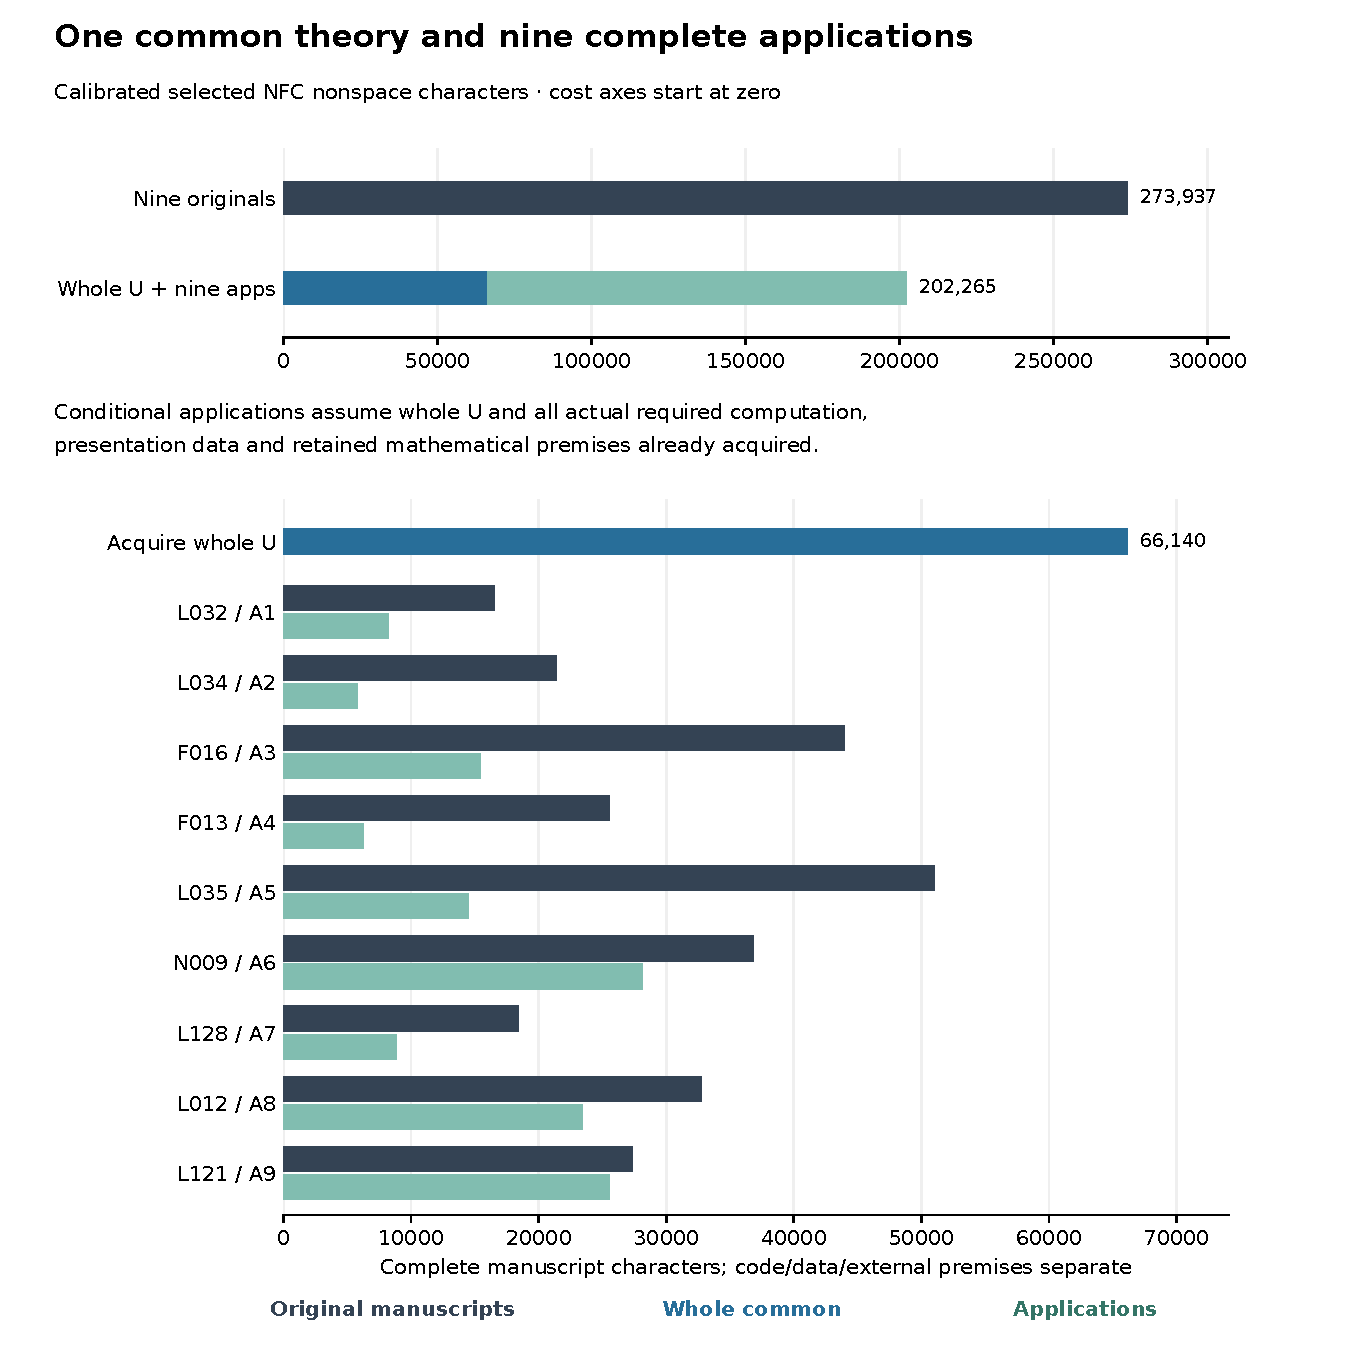
\includegraphics[width=\textwidth]{costs.pdf}\end{center}
The upper chart pays the whole common paper and each complete application. The lower chart displays the same common acquisition cost and every source/application pair. All 30 rectangles have areas proportional to manuscript length at their chart's fixed height; cost axes begin at zero. They represent text costs, not ratios or theorem counts.

Executable code is excluded symmetrically from the written comparison. Mathematical proofs, algorithms described in prose, presentations and tables remain. Required programs and data remain premises despite being outside this manuscript-only scalar. Historical source software is unknown, so there is no software-inclusive or optional-validation-inclusive factor.
\newpage
\begin{center}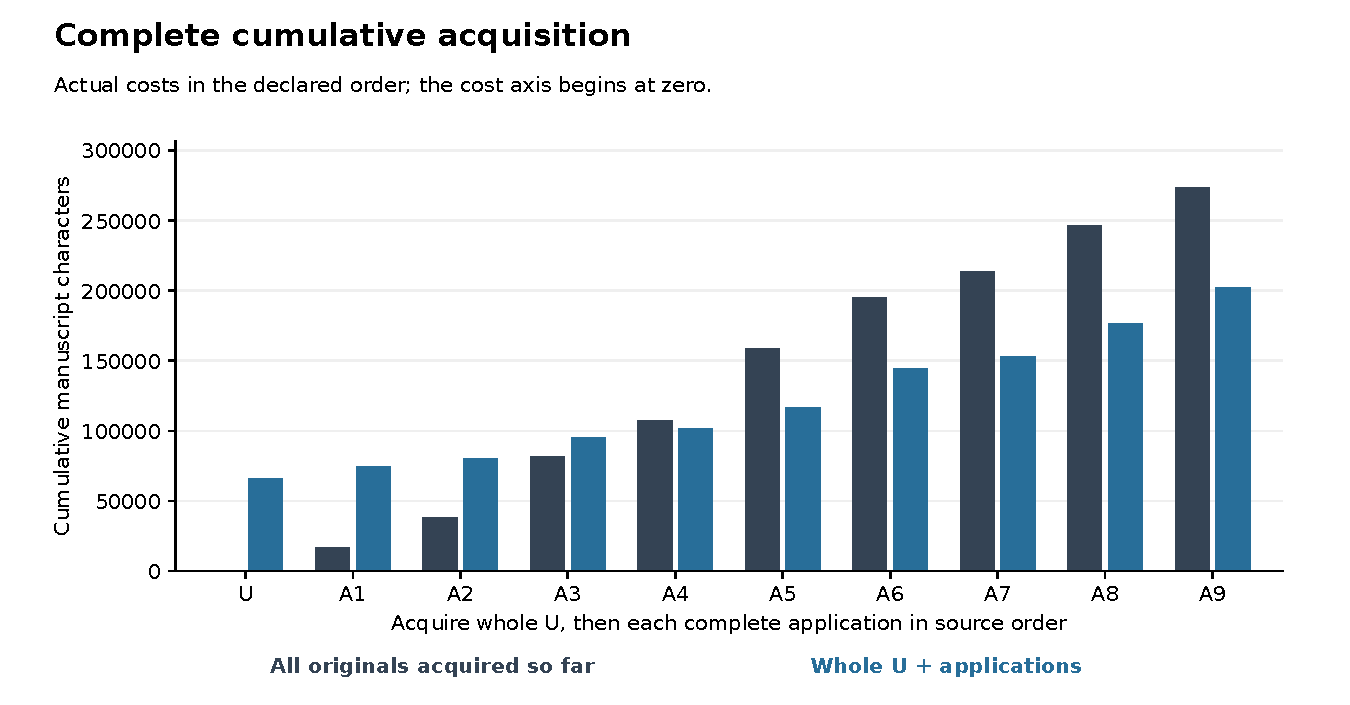
\includegraphics[width=\textwidth]{cumulative.pdf}\end{center}
Stage zero acquires all of $U$. Each later stage adds one complete source on the historical side and its complete application on our side. These ten cumulative stages use the inherited documentary order followed by L121. No optimal order or general sawtooth behavior is asserted. Required computation, data and external proofs remain separately acquired obligations.

\textbf{Complete separate file inventory.}
\begin{center}\small\begin{tabular}{lrrr}\toprule
Whole files & Count & NFC nonspace & Literal bytes\\\midrule
Required programs and data & 20 & 92,586 & 105,850\\
Inherited auxiliaries & 3 & 16,581 & 18,741\\
Operational runners & 6 & 26,056 & 28,439\\
Partial formal files & 16 & 70,785 & 100,644\\
\bottomrule\end{tabular}\end{center}
All 45 contents are distinct and fully inventoried. The twenty mathematical files comprise the eleven old required files and L121's eight programs plus mandatory \texttt{model\_data.json}. In particular \path{cubic_relation/check.py} is a required calculation. Six operational runners and three auxiliaries remain separate. The sixteen formal files are fifteen Lean modules and one dependency manifest; all formal scopes remain partial.

The three old printed appendices total 30 pages and represent only the old eleven-file mathematical collection. Their primary text costs are 53,035, 17,250 and 1,175 characters. No complete printed representation exists for the enlarged twenty-file collection. These partial printed costs are not added to raw files, nor used for a whole-program factor. Historical software and retained external proof costs remain unknown, not zero.
\newpage
\textbf{Sensitivity of the whole written factor.}
\begin{center}\small\begin{tabular}{lrrr}\toprule
Unit & Raw complete & Raw selected & Calibrated\\\midrule
NFC: Whitespace tokens & 1.575336 & 1.562663 & 1.562686\\
NFC: Alphanumeric units & 1.659216 & 1.643929 & 1.643605\\
NFC: Nonspace characters & 1.368839 & 1.354312 & 1.354347\\
NFC: Collapsed-space characters & 1.405302 & 1.391061 & 1.391094\\
NFC: Collapsed UTF-8 bytes & 1.344251 & 1.331315 & 1.332857\\
NFKC: Whitespace tokens & 1.577578 & 1.564911 & 1.564934\\
NFKC: Alphanumeric units & 1.659216 & 1.643929 & 1.643605\\
NFKC: Nonspace characters & 1.370236 & 1.355716 & 1.355750\\
NFKC: Collapsed-space characters & 1.406838 & 1.392603 & 1.392636\\
NFKC: Collapsed UTF-8 bytes & 1.458205 & 1.444239 & 1.444673\\
\bottomrule\end{tabular}\end{center}
All 30 coordinates and 300 exact fractions are supplied in JSON and CSV: one whole-topic and nine conditional comparisons in each coordinate. Every fraction records its complete unreduced source and replacement costs, reduced numerator and denominator, and a twelve-place decimal. The 240 previous conditional fraction records are preserved exactly. All 660 PDF input cells and 450 complete raw-file cells are unchanged from the adopted inputs.

Raw complete extraction retains running furniture. Selection removes only the exact accepted furniture; calibration applies occurrence-bound actual glyph repairs. Ordinary printed hyphens and ligatures remain, and NFKC is a separate sensitivity. The new source contributes twelve whole pages and its replacement eleven. Neither contains an executable listing. The 18 source and 51 application glyph repairs and all earlier source calibrations are the adopted input layer, not new decisions in this numerical calculation.

\textbf{Scientific and measurement limits.} The 102 earlier dispositions and L121's 27 corrected dispositions remain unchanged: nine original manuscripts, not 129 originals. The L121 corrections, retained Euclidean Coxeter and toroidal inputs, and all prior source qualifications remain in force. Numerical comparison adds no source, theorem, question or formalization credit.

L035's unextracted image labels on physical pages 9, 10, 12 and 22 remain unmeasured. L121's vector diagrams on pages 5--7 retain extracted labels but not priced graphical structure. Full graphics/layout, retained external proof libraries, installed software/databases, historical programs/data and complete formalization costs are unknown. The six added Lean declarations verify countermodel relations and two nonconsequences only; they do not formalize group orders, infinite families or geometry.

The numerical author previously reviewed these inputs and contributed to earlier affine work. Input authoring, scientific acceptance and root input adoption are separately bound; earlier numerical mechanics are reused with attribution. This packet performs no new extraction, mathematical enumeration or Lean compilation. A distinct numerical review is required before public admission.
\end{document}
